\documentclass{article}
\usepackage[T1]{fontenc}
\usepackage[utf8]{inputenc}
\usepackage{url}
\usepackage{listings}
\usepackage{tikz}
\usepackage{float}

\lstset{
  basicstyle=\ttfamily\footnotesize,
  breaklines=true,
  breakatwhitespace=false,
  columns=fullflexible,
  keepspaces=true
}

\tikzset{
  vertex/.style={circle, draw, minimum size=8mm, inner sep=0pt},
  frontier/.style={circle, draw, fill=blue!25, minimum size=8mm, inner sep=0pt},
  visited/.style={circle, draw, fill=gray!25, minimum size=8mm, inner sep=0pt},
  undiscovered/.style={circle, draw, fill=white, minimum size=8mm, inner sep=0pt},
  treeedge/.style={very thick, blue!70!black},
  graphedge/.style={gray!70}
}

\begin{document}

\section{BFS}
A Busca em Largura, ou \textit{Breadth-First Search} (BFS), é um dos algoritmos fundamentais de travessia em grafos \cite{cormenalgorithms}. O algoritmo parte de um vértice inicial e, em seguida, visita os demais vértices em camadas, primeiro os que estão a uma aresta de distância, depois os que estão a duas arestas, e assim sucessivamente. Dessa forma, em um grafo não ponderado, a BFS calcula a menor distância, em número de arestas, entre o vértice inicial e todos os vértices alcançáveis a partir dele. A Busca em Largura também gera uma árvore chamada \textit{Árvore de Busca em Largura}, na qual o pai de um vértice é aquele que o descobriu durante a busca.

A implementação clássica utiliza uma fila. O vértice inicial é inserido na fila, marcado como visitado, e sua distância é definida como zero. Em seguida, enquanto a fila não estiver vazia, repete-se a seguinte operação retira-se um vértice $v$ da fila e examinam-se todos os vértices $u$ vizinhos de $v$. Caso $u$ ainda não tenha sido visitado, sua distância é calculada, ele é marcado como visitado e adicionado à fila.

Uma forma simplificada do algoritmo é apresentada a seguir:

\begin{lstlisting}
BFS(G, origem):
	para cada vertice v em G:
        pai[v] = none

    pai[origem] = origem
    fila = {origem}

    enquanto fila nao esta vazia:
		u = proximo elemento da fila
		para cada vizinho v de u:
			se pai[v] == none:
				pai[v] = u
				adiciona v na fila
\end{lstlisting}

\subsection{BFS em Fronteiras}
O algoritmo de BFS também pode ser implementado como uma descoberta por fronteiras. Inicializa-se a primeira fronteira com o vértice inicial. Em seguida, para cada vértice presente na fronteira atual, examinam-se todos os seus vizinhos; aqueles que ainda não foram visitados são adicionados à próxima fronteira. Esse processo se repete sucessivamente, até que a fronteira atual esteja vazia.

Uma versão simplificada do algoritmo é apresentada a seguir:

\begin{lstlisting}
BFS(G, origem):
    para cada vertice v em G:
        pai[v] = none

    pai[origem] = origem
    fronteira = {origem}

    enquanto fronteira nao esta vazia:
        proxima_fronteira = vazia
        para cada vertice u na fronteira:
            para cada vizinho v de u:
                se pai[v] == none:
                    pai[v] = u
                    adiciona v na proxima_fronteira
        fronteira = proxima_fronteira
\end{lstlisting}

\subsection{Exemplo Visual de Fronteiras}

Considere o grafo da Figura~\ref{fig:bfs-step0}. A busca comeca no vertice
\texttt{A}. Em cada passo, os vertices em azul representam a fronteira atual,
os vertices em cinza ja foram visitados em niveis anteriores, e os vertices em
branco ainda nao foram descobertos. As arestas destacadas em azul formam a
arvore de BFS construida ate aquele momento. Essa arvore registra, para cada
vertice descoberto, qual foi o vertice responsavel por sua primeira descoberta.
Assim, cada aresta azul liga um vertice ao seu pai na busca, permitindo recuperar
um caminho minimo, em numero de arestas, da origem \texttt{A} ate qualquer
vertice alcancavel.

\begin{figure}[H]
\centering
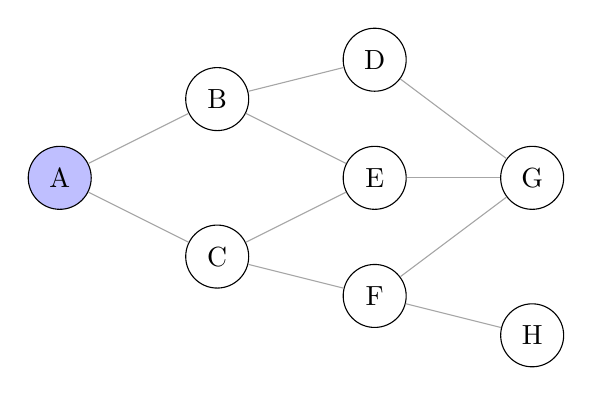
\begin{tikzpicture}[scale=1.0]
  \node[frontier] (A) at (0,0) {A};
  \node[undiscovered] (B) at (2,1) {B};
  \node[undiscovered] (C) at (2,-1) {C};
  \node[undiscovered] (D) at (4,1.5) {D};
  \node[undiscovered] (E) at (4,0) {E};
  \node[undiscovered] (F) at (4,-1.5) {F};
  \node[undiscovered] (G) at (6,0) {G};
  \node[undiscovered] (H) at (6,-2) {H};

  \draw[graphedge] (A) -- (B);
  \draw[graphedge] (A) -- (C);
  \draw[graphedge] (B) -- (D);
  \draw[graphedge] (B) -- (E);
  \draw[graphedge] (C) -- (E);
  \draw[graphedge] (C) -- (F);
  \draw[graphedge] (D) -- (G);
  \draw[graphedge] (E) -- (G);
  \draw[graphedge] (F) -- (G);
  \draw[graphedge] (F) -- (H);
\end{tikzpicture}
\caption{Passo 0 da BFS: a fronteira inicial contem apenas a origem \texttt{A}.}
\label{fig:bfs-step0}
\end{figure}

No passo inicial, a distancia de \texttt{A} e zero. A primeira expansao examina
as arestas que saem de \texttt{A}. Como \texttt{B} e \texttt{C} ainda nao foram
visitados, ambos sao descobertos, recebem distancia um e passam a formar a
proxima fronteira.

\begin{figure}[H]
\centering
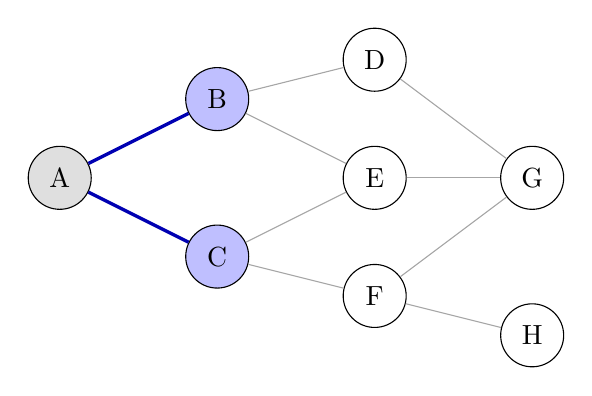
\begin{tikzpicture}[scale=1.0]
  \node[visited] (A) at (0,0) {A};
  \node[frontier] (B) at (2,1) {B};
  \node[frontier] (C) at (2,-1) {C};
  \node[undiscovered] (D) at (4,1.5) {D};
  \node[undiscovered] (E) at (4,0) {E};
  \node[undiscovered] (F) at (4,-1.5) {F};
  \node[undiscovered] (G) at (6,0) {G};
  \node[undiscovered] (H) at (6,-2) {H};

  \draw[treeedge] (A) -- (B);
  \draw[treeedge] (A) -- (C);
  \draw[graphedge] (B) -- (D);
  \draw[graphedge] (B) -- (E);
  \draw[graphedge] (C) -- (E);
  \draw[graphedge] (C) -- (F);
  \draw[graphedge] (D) -- (G);
  \draw[graphedge] (E) -- (G);
  \draw[graphedge] (F) -- (G);
  \draw[graphedge] (F) -- (H);
\end{tikzpicture}
\caption{Passo 1 da BFS: \texttt{B} e \texttt{C} formam a fronteira de nivel 1.}
\label{fig:bfs-step1}
\end{figure}

No segundo passo, a BFS expande todos os vertices da fronteira atual. O vertice
\texttt{B} descobre \texttt{D} e \texttt{E}. O vertice \texttt{C} tambem possui
uma aresta para \texttt{E}, mas \texttt{E} ja pode ter sido descoberto por
\texttt{B}; nesse caso, a implementacao mantem apenas um pai para \texttt{E}.
O vertice \texttt{C} tambem descobre \texttt{F}. Assim, a nova fronteira passa a
ser formada por \texttt{D}, \texttt{E} e \texttt{F}, todos com distancia dois.

\begin{figure}[H]
\centering
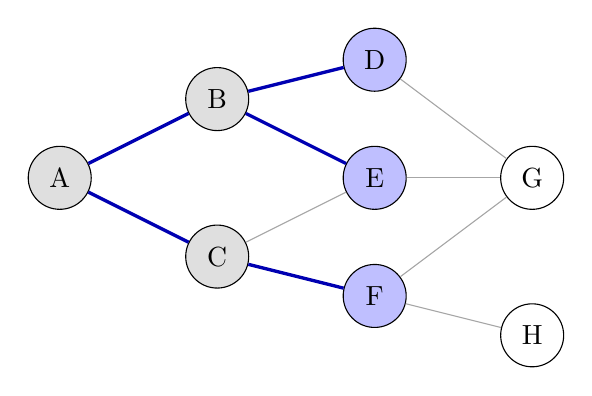
\begin{tikzpicture}[scale=1.0]
  \node[visited] (A) at (0,0) {A};
  \node[visited] (B) at (2,1) {B};
  \node[visited] (C) at (2,-1) {C};
  \node[frontier] (D) at (4,1.5) {D};
  \node[frontier] (E) at (4,0) {E};
  \node[frontier] (F) at (4,-1.5) {F};
  \node[undiscovered] (G) at (6,0) {G};
  \node[undiscovered] (H) at (6,-2) {H};

  \draw[treeedge] (A) -- (B);
  \draw[treeedge] (A) -- (C);
  \draw[treeedge] (B) -- (D);
  \draw[treeedge] (B) -- (E);
  \draw[graphedge] (C) -- (E);
  \draw[treeedge] (C) -- (F);
  \draw[graphedge] (D) -- (G);
  \draw[graphedge] (E) -- (G);
  \draw[graphedge] (F) -- (G);
  \draw[graphedge] (F) -- (H);
\end{tikzpicture}
\caption{Passo 2 da BFS: \texttt{D}, \texttt{E} e \texttt{F} formam a fronteira de nivel 2.}
\label{fig:bfs-step2}
\end{figure}

No terceiro passo, a fronteira de nivel dois e expandida. Os vertices
\texttt{D}, \texttt{E} e \texttt{F} possuem arestas para \texttt{G}. O primeiro
que conseguir registrar \texttt{G} como descoberto define seu pai na arvore de
BFS. Na figura, \texttt{E} foi escolhido como pai de \texttt{G}, mas
\texttt{D} ou \texttt{F} tambem poderiam ser pais validos, pois todos pertencem
ao nivel anterior. Alem disso, \texttt{F} descobre \texttt{H}, que tambem passa
a fazer parte da fronteira de nivel tres.

\begin{figure}[H]
\centering
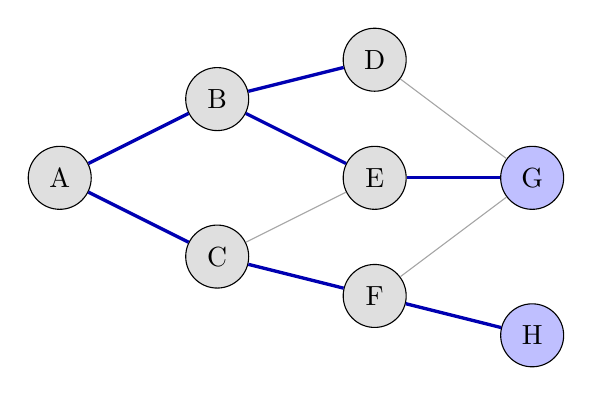
\begin{tikzpicture}[scale=1.0]
  \node[visited] (A) at (0,0) {A};
  \node[visited] (B) at (2,1) {B};
  \node[visited] (C) at (2,-1) {C};
  \node[visited] (D) at (4,1.5) {D};
  \node[visited] (E) at (4,0) {E};
  \node[visited] (F) at (4,-1.5) {F};
  \node[frontier] (G) at (6,0) {G};
  \node[frontier] (H) at (6,-2) {H};

  \draw[treeedge] (A) -- (B);
  \draw[treeedge] (A) -- (C);
  \draw[treeedge] (B) -- (D);
  \draw[treeedge] (B) -- (E);
  \draw[graphedge] (C) -- (E);
  \draw[treeedge] (C) -- (F);
  \draw[graphedge] (D) -- (G);
  \draw[treeedge] (E) -- (G);
  \draw[graphedge] (F) -- (G);
  \draw[treeedge] (F) -- (H);
\end{tikzpicture}
\caption{Passo 3 da BFS: \texttt{G} e \texttt{H} sao descobertos no nivel 3.}
\label{fig:bfs-step3}
\end{figure}

Depois da expansao de \texttt{G}, nenhum novo vertice e encontrado. A proxima
fronteira fica vazia e o algoritmo termina. O resultado e uma arvore de BFS na
qual cada vertice alcancavel possui um pai em um nivel imediatamente anterior ao
seu.

\subsection{Motivacao de Paralelismo}
A BFS baseada em fronteiras oferece uma oportunidade natural de paralelismo, todos
os vertices de uma mesma fronteira podem ser processados simultaneamente, e suas
arestas podem ser expandidas em paralelo. O principal cuidado e controlar a
descoberta dos vertices da proxima fronteira, pois multiplas arestas podem tentar
descobrir o mesmo vertice ao mesmo tempo. Estrategias de paralelismo e controle foram
discultidas em \cite{merrillgpu}. 

\subsection{Divisão do Grafo entre Workers}
Neste texto, o termo \textit{worker} e usado de forma geral para representar uma
unidade de execucao capaz de armazenar parte do grafo e realizar parte do trabalho
da BFS. Um worker pode corresponder, por exemplo, a um processo, uma maquina, uma
GPU, uma CPU ou outro recurso de execucao paralelo. Os detalhes de como esses
workers sao implementados serao discutidos posteriormente. Essa abstracao e
comum em sistemas de processamento paralelo de grafos, nos quais a computacao e
dividida entre unidades que armazenam partes do grafo e trocam informacoes sobre
vertices descobertos durante a execucao \cite{merrillgpu}.

Em uma implementação paralela ou distribuída, o grafo não precisa ficar inteiro
em uma única unidade de execução. Uma estratégia comum é dividir seus vértices entre vários
\textit{workers}. Cada worker fica responsável por armazenar e processar uma
parte dos vértices e de suas listas de adjacência. Durante a BFS, quando um
worker expande um vértice local, ele examina suas arestas; se o vizinho pertence
a outro worker, a descoberta desse vizinho precisa ser comunicada ao worker que
o possui \cite{merrillgpu}.

Uma forma simples de particionamento é a distribuição cíclica. Com $n_workers$
workers, o dono de um vértice pode ser calculado por:

\begin{lstlisting}
worker(v) = v mod n_workers
\end{lstlisting}

Assim, os vértices são distribuídos de maneira alternada entre os workers. Essa
estratégia não garante balanceamento perfeito para todos os grafos, mas é simples
e evita concentrar intervalos inteiros de vértices em um único worker. A
Tabela~\ref{tab:worker-partition} mostra um exemplo com 16 vértices.

\begin{table}[H]
\centering
\begin{tabular}{c|c}
Worker & Vértices pertencentes ao worker \\
\hline
0 & 0, 4, 8, 12 \\
1 & 1, 5, 9, 13 \\
2 & 2, 6, 10, 14 \\
3 & 3, 7, 11, 15 \\
\end{tabular}
\caption{Particionamento cíclico de 16 vértices entre 4 workers.}
\label{tab:worker-partition}
\end{table}

A Figura~\ref{fig:grafo-global-workers} mostra a visão global de um grafo com 16
vértices. Essa visão representa o grafo completo antes de considerar qual worker
é responsável por cada vértice.

\begin{figure}[H]
\centering
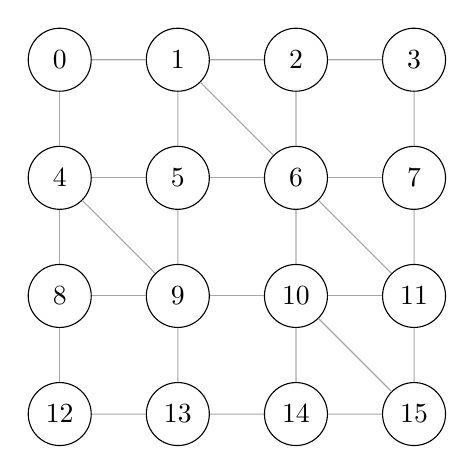
\begin{tikzpicture}[scale=0.75]
  \foreach \i/\x/\y in {0/0/3,1/2/3,2/4/3,3/6/3,
                        4/0/1,5/2/1,6/4/1,7/6/1,
                        8/0/-1,9/2/-1,10/4/-1,11/6/-1,
                        12/0/-3,13/2/-3,14/4/-3,15/6/-3} {
    \node[vertex] (v\i) at (\x,\y) {\i};
  }

  \draw[graphedge] (v0) -- (v1);
  \draw[graphedge] (v1) -- (v2);
  \draw[graphedge] (v2) -- (v3);
  \draw[graphedge] (v0) -- (v4);
  \draw[graphedge] (v1) -- (v5);
  \draw[graphedge] (v2) -- (v6);
  \draw[graphedge] (v3) -- (v7);
  \draw[graphedge] (v4) -- (v5);
  \draw[graphedge] (v5) -- (v6);
  \draw[graphedge] (v6) -- (v7);
  \draw[graphedge] (v4) -- (v8);
  \draw[graphedge] (v5) -- (v9);
  \draw[graphedge] (v6) -- (v10);
  \draw[graphedge] (v7) -- (v11);
  \draw[graphedge] (v8) -- (v9);
  \draw[graphedge] (v9) -- (v10);
  \draw[graphedge] (v10) -- (v11);
  \draw[graphedge] (v8) -- (v12);
  \draw[graphedge] (v9) -- (v13);
  \draw[graphedge] (v10) -- (v14);
  \draw[graphedge] (v11) -- (v15);
  \draw[graphedge] (v12) -- (v13);
  \draw[graphedge] (v13) -- (v14);
  \draw[graphedge] (v14) -- (v15);
  \draw[graphedge] (v1) -- (v6);
  \draw[graphedge] (v4) -- (v9);
  \draw[graphedge] (v6) -- (v11);
  \draw[graphedge] (v10) -- (v15);
\end{tikzpicture}
\caption{Visão global de um grafo com 16 vértices antes do particionamento.}
\label{fig:grafo-global-workers}
\end{figure}

A Figura~\ref{fig:grafo-particionado-workers} mostra o mesmo grafo particionado
entre quatro workers. As cores indicam o dono de cada vértice. As arestas que
ligam vértices de cores diferentes representam comunicações potenciais durante a
BFS, pois a expansão de um vértice em um worker pode descobrir um vértice que
pertence a outro worker.

\begin{figure}[H]
\centering
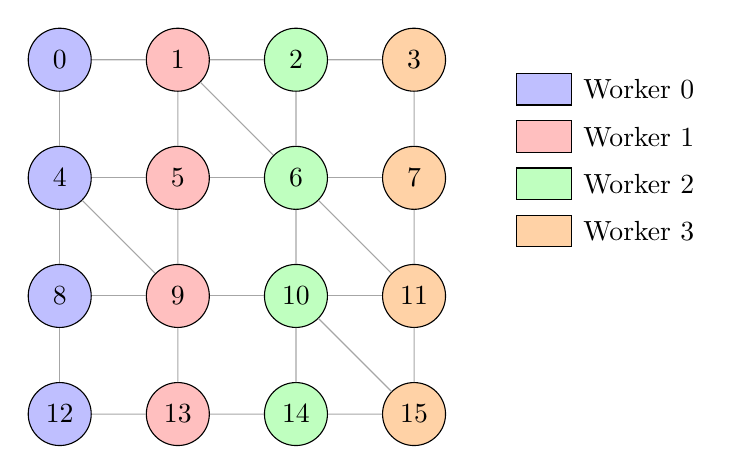
\begin{tikzpicture}[scale=0.75]
  \foreach \i/\x/\y/\c in {0/0/3/blue!25,1/2/3/red!25,2/4/3/green!25,3/6/3/orange!35,
                           4/0/1/blue!25,5/2/1/red!25,6/4/1/green!25,7/6/1/orange!35,
                           8/0/-1/blue!25,9/2/-1/red!25,10/4/-1/green!25,11/6/-1/orange!35,
                           12/0/-3/blue!25,13/2/-3/red!25,14/4/-3/green!25,15/6/-3/orange!35} {
    \node[circle, draw, fill=\c, minimum size=8mm, inner sep=0pt] (p\i) at (\x,\y) {\i};
  }

  \draw[graphedge] (p0) -- (p1);
  \draw[graphedge] (p1) -- (p2);
  \draw[graphedge] (p2) -- (p3);
  \draw[graphedge] (p0) -- (p4);
  \draw[graphedge] (p1) -- (p5);
  \draw[graphedge] (p2) -- (p6);
  \draw[graphedge] (p3) -- (p7);
  \draw[graphedge] (p4) -- (p5);
  \draw[graphedge] (p5) -- (p6);
  \draw[graphedge] (p6) -- (p7);
  \draw[graphedge] (p4) -- (p8);
  \draw[graphedge] (p5) -- (p9);
  \draw[graphedge] (p6) -- (p10);
  \draw[graphedge] (p7) -- (p11);
  \draw[graphedge] (p8) -- (p9);
  \draw[graphedge] (p9) -- (p10);
  \draw[graphedge] (p10) -- (p11);
  \draw[graphedge] (p8) -- (p12);
  \draw[graphedge] (p9) -- (p13);
  \draw[graphedge] (p10) -- (p14);
  \draw[graphedge] (p11) -- (p15);
  \draw[graphedge] (p12) -- (p13);
  \draw[graphedge] (p13) -- (p14);
  \draw[graphedge] (p14) -- (p15);
  \draw[graphedge] (p1) -- (p6);
  \draw[graphedge] (p4) -- (p9);
  \draw[graphedge] (p6) -- (p11);
  \draw[graphedge] (p10) -- (p15);

  \node[draw, fill=blue!25, minimum width=7mm, minimum height=4mm] at (8.2,2.5) {};
  \node[anchor=west] at (8.7,2.5) {Worker 0};
  \node[draw, fill=red!25, minimum width=7mm, minimum height=4mm] at (8.2,1.7) {};
  \node[anchor=west] at (8.7,1.7) {Worker 1};
  \node[draw, fill=green!25, minimum width=7mm, minimum height=4mm] at (8.2,0.9) {};
  \node[anchor=west] at (8.7,0.9) {Worker 2};
  \node[draw, fill=orange!35, minimum width=7mm, minimum height=4mm] at (8.2,0.1) {};
  \node[anchor=west] at (8.7,0.1) {Worker 3};
\end{tikzpicture}
\caption{Mesmo grafo particionado entre 4 workers usando a regra $worker(v) = v \bmod 4$.}
\label{fig:grafo-particionado-workers}
\end{figure}

\subsection{Exemplo de BFS Paralela com 4 Workers}
Considere uma BFS iniciada no vértice 0 do grafo particionado da
Figura~\ref{fig:grafo-particionado-workers}. No passo inicial, apenas o worker 0
possui trabalho, pois ele é o dono do vértice 0. Ao expandir 0, são descobertos
os vértices 1 e 4. O vértice 4 pertence ao próprio worker 0, enquanto o vértice 1
pertence ao worker 1. Portanto, a nova fronteira já fica distribuída entre mais
de um worker.

Após a expansão dos vértices 1 e 4, a BFS chega ao passo mostrado na
Figura~\ref{fig:bfs-paralela-step2}. Nesse momento, a fronteira global de
nível 2 é formada por vértices armazenados em workers diferentes. O worker 0
possui o vértice 8 na fronteira, o worker 1 possui os vértices 5 e 9, o worker 2
possui os vértices 2 e 6, e o worker 3 ainda não possui vértices na fronteira
atual.

A expansão passo a passo é mostrada nas figuras seguintes. Em cada uma delas, a
fronteira global é dividida entre os quatro workers. Os vértices em azul formam
a fronteira local do passo atual, os vértices em cinza já foram visitados, e os
vértices em branco ainda não foram descobertos. Depois que todos os workers
expandem suas fronteiras locais, os vértices recém-descobertos formam a
fronteira do próximo nível.

No passo 0, apenas o worker 0 possui trabalho, pois a origem 0 pertence a ele.

\begin{figure}[H]
\centering
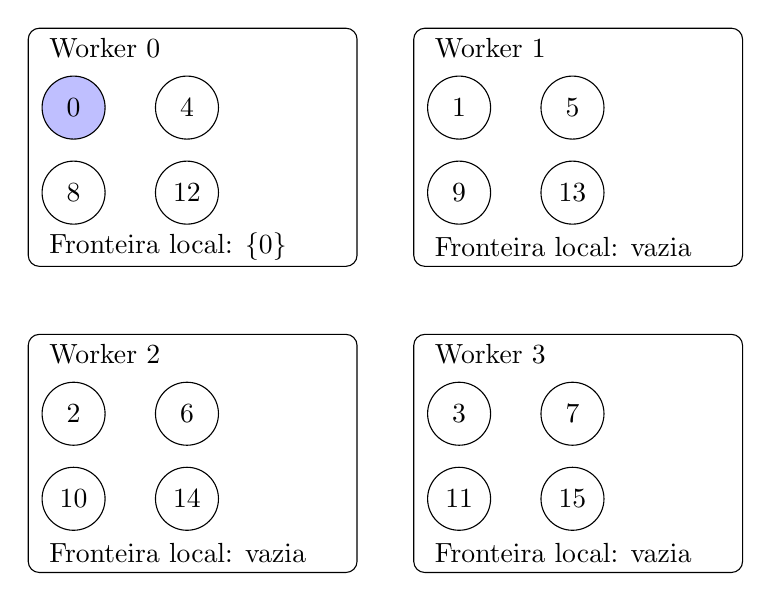
\begin{tikzpicture}[scale=0.72]
  \draw[rounded corners] (-0.8,-0.8) rectangle (5.0,3.4);
  \node[anchor=west] at (-0.6,3.05) {Worker 0};
  \node[frontier] (s0w0v0) at (0,2) {0};
  \node[undiscovered] (s0w0v4) at (2,2) {4};
  \node[undiscovered] (s0w0v8) at (0,0.5) {8};
  \node[undiscovered] (s0w0v12) at (2,0.5) {12};
  \node[anchor=west] at (-0.6,-0.45) {Fronteira local: \{0\}};

  \draw[rounded corners] (6.0,-0.8) rectangle (11.8,3.4);
  \node[anchor=west] at (6.2,3.05) {Worker 1};
  \node[undiscovered] at (6.8,2) {1};
  \node[undiscovered] at (8.8,2) {5};
  \node[undiscovered] at (6.8,0.5) {9};
  \node[undiscovered] at (8.8,0.5) {13};
  \node[anchor=west] at (6.2,-0.45) {Fronteira local: vazia};

  \draw[rounded corners] (-0.8,-6.2) rectangle (5.0,-2.0);
  \node[anchor=west] at (-0.6,-2.35) {Worker 2};
  \node[undiscovered] at (0,-3.4) {2};
  \node[undiscovered] at (2,-3.4) {6};
  \node[undiscovered] at (0,-4.9) {10};
  \node[undiscovered] at (2,-4.9) {14};
  \node[anchor=west] at (-0.6,-5.85) {Fronteira local: vazia};

  \draw[rounded corners] (6.0,-6.2) rectangle (11.8,-2.0);
  \node[anchor=west] at (6.2,-2.35) {Worker 3};
  \node[undiscovered] at (6.8,-3.4) {3};
  \node[undiscovered] at (8.8,-3.4) {7};
  \node[undiscovered] at (6.8,-4.9) {11};
  \node[undiscovered] at (8.8,-4.9) {15};
  \node[anchor=west] at (6.2,-5.85) {Fronteira local: vazia};
\end{tikzpicture}
\caption{Passo 0 da BFS paralela: apenas a origem 0 está na fronteira.}
\label{fig:bfs-paralela-step0}
\end{figure}

Ao expandir 0, são descobertos 1 e 4. O vértice 4 permanece no worker 0, e o
vértice 1 passa a compor a fronteira local do worker 1.

\begin{figure}[H]
\centering
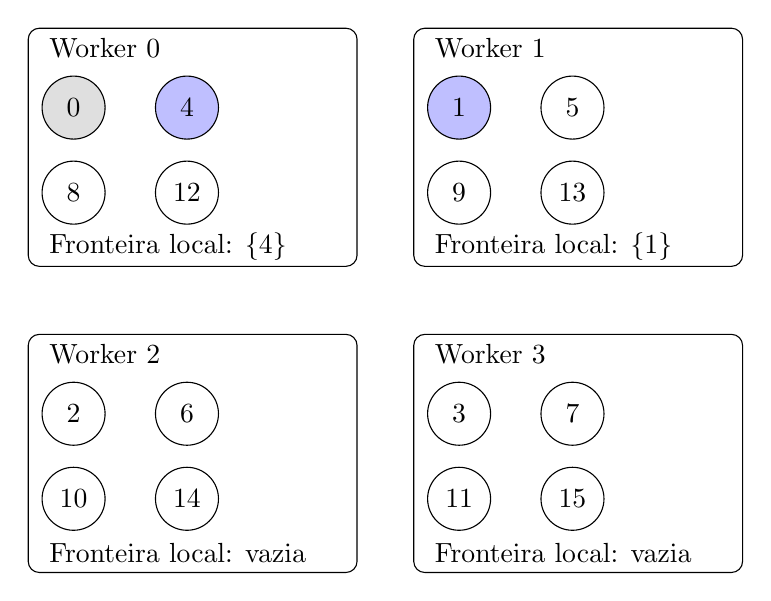
\begin{tikzpicture}[scale=0.72]
  \draw[rounded corners] (-0.8,-0.8) rectangle (5.0,3.4);
  \node[anchor=west] at (-0.6,3.05) {Worker 0};
  \node[visited] at (0,2) {0};
  \node[frontier] at (2,2) {4};
  \node[undiscovered] at (0,0.5) {8};
  \node[undiscovered] at (2,0.5) {12};
  \node[anchor=west] at (-0.6,-0.45) {Fronteira local: \{4\}};

  \draw[rounded corners] (6.0,-0.8) rectangle (11.8,3.4);
  \node[anchor=west] at (6.2,3.05) {Worker 1};
  \node[frontier] at (6.8,2) {1};
  \node[undiscovered] at (8.8,2) {5};
  \node[undiscovered] at (6.8,0.5) {9};
  \node[undiscovered] at (8.8,0.5) {13};
  \node[anchor=west] at (6.2,-0.45) {Fronteira local: \{1\}};

  \draw[rounded corners] (-0.8,-6.2) rectangle (5.0,-2.0);
  \node[anchor=west] at (-0.6,-2.35) {Worker 2};
  \node[undiscovered] at (0,-3.4) {2};
  \node[undiscovered] at (2,-3.4) {6};
  \node[undiscovered] at (0,-4.9) {10};
  \node[undiscovered] at (2,-4.9) {14};
  \node[anchor=west] at (-0.6,-5.85) {Fronteira local: vazia};

  \draw[rounded corners] (6.0,-6.2) rectangle (11.8,-2.0);
  \node[anchor=west] at (6.2,-2.35) {Worker 3};
  \node[undiscovered] at (6.8,-3.4) {3};
  \node[undiscovered] at (8.8,-3.4) {7};
  \node[undiscovered] at (6.8,-4.9) {11};
  \node[undiscovered] at (8.8,-4.9) {15};
  \node[anchor=west] at (6.2,-5.85) {Fronteira local: vazia};
\end{tikzpicture}
\caption{Passo 1 da BFS paralela: os workers 0 e 1 possuem vértices na fronteira.}
\label{fig:bfs-paralela-step1}
\end{figure}

No passo 1, os workers 0 e 1 trabalham ao mesmo tempo: 4 descobre 8 e 9,
enquanto 1 descobre 2, 5 e 6. O vértice 5 também é vizinho de 4, mas basta que
uma das tentativas de descoberta seja aceita para que ele entre na próxima
fronteira. No passo 2, já há trabalho em três workers diferentes.

\begin{figure}[H]
\centering
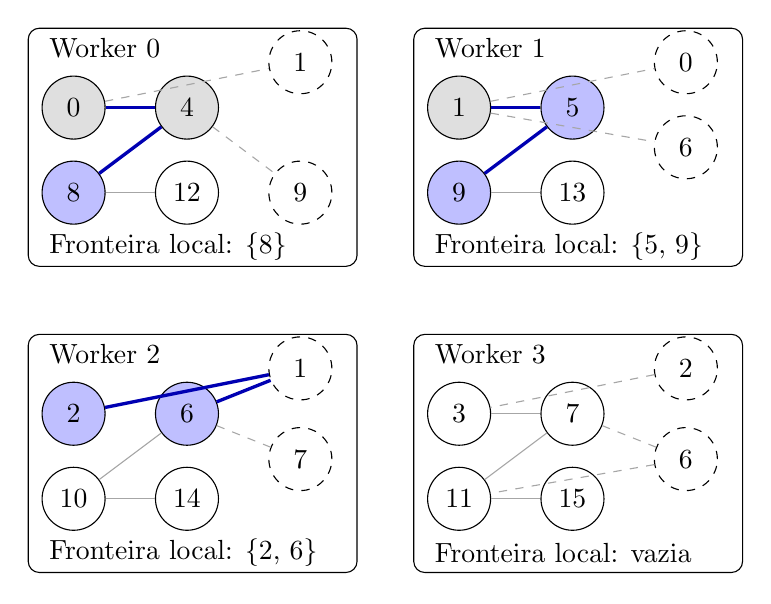
\begin{tikzpicture}[scale=0.72]
  \draw[rounded corners] (-0.8,-0.8) rectangle (5.0,3.4);
  \node[anchor=west] at (-0.6,3.05) {Worker 0};
  \node[visited] (w0v0) at (0,2) {0};
  \node[visited] (w0v4) at (2,2) {4};
  \node[frontier] (w0v8) at (0,0.5) {8};
  \node[undiscovered] (w0v12) at (2,0.5) {12};
  \node[draw, dashed, circle, minimum size=8mm, inner sep=0pt] (w0g1) at (4,2.8) {1};
  \node[draw, dashed, circle, minimum size=8mm, inner sep=0pt] (w0g9) at (4,0.5) {9};
  \draw[treeedge] (w0v0) -- (w0v4);
  \draw[treeedge] (w0v4) -- (w0v8);
  \draw[graphedge] (w0v8) -- (w0v12);
  \draw[graphedge, dashed] (w0v0) -- (w0g1);
  \draw[graphedge, dashed] (w0v4) -- (w0g9);
  \node[anchor=west] at (-0.6,-0.45) {Fronteira local: \{8\}};

  \draw[rounded corners] (6.0,-0.8) rectangle (11.8,3.4);
  \node[anchor=west] at (6.2,3.05) {Worker 1};
  \node[visited] (w1v1) at (6.8,2) {1};
  \node[frontier] (w1v5) at (8.8,2) {5};
  \node[frontier] (w1v9) at (6.8,0.5) {9};
  \node[undiscovered] (w1v13) at (8.8,0.5) {13};
  \node[draw, dashed, circle, minimum size=8mm, inner sep=0pt] (w1g0) at (10.8,2.8) {0};
  \node[draw, dashed, circle, minimum size=8mm, inner sep=0pt] (w1g6) at (10.8,1.3) {6};
  \draw[treeedge] (w1v1) -- (w1v5);
  \draw[treeedge] (w1v5) -- (w1v9);
  \draw[graphedge] (w1v9) -- (w1v13);
  \draw[graphedge, dashed] (w1v1) -- (w1g0);
  \draw[graphedge, dashed] (w1v1) -- (w1g6);
  \node[anchor=west] at (6.2,-0.45) {Fronteira local: \{5, 9\}};

  \draw[rounded corners] (-0.8,-6.2) rectangle (5.0,-2.0);
  \node[anchor=west] at (-0.6,-2.35) {Worker 2};
  \node[frontier] (w2v2) at (0,-3.4) {2};
  \node[frontier] (w2v6) at (2,-3.4) {6};
  \node[undiscovered] (w2v10) at (0,-4.9) {10};
  \node[undiscovered] (w2v14) at (2,-4.9) {14};
  \node[draw, dashed, circle, minimum size=8mm, inner sep=0pt] (w2g1) at (4,-2.6) {1};
  \node[draw, dashed, circle, minimum size=8mm, inner sep=0pt] (w2g7) at (4,-4.2) {7};
  \draw[treeedge] (w2g1) -- (w2v2);
  \draw[treeedge] (w2g1) -- (w2v6);
  \draw[graphedge] (w2v6) -- (w2v10);
  \draw[graphedge] (w2v10) -- (w2v14);
  \draw[graphedge, dashed] (w2v6) -- (w2g7);
  \node[anchor=west] at (-0.6,-5.85) {Fronteira local: \{2, 6\}};

  \draw[rounded corners] (6.0,-6.2) rectangle (11.8,-2.0);
  \node[anchor=west] at (6.2,-2.35) {Worker 3};
  \node[undiscovered] (w3v3) at (6.8,-3.4) {3};
  \node[undiscovered] (w3v7) at (8.8,-3.4) {7};
  \node[undiscovered] (w3v11) at (6.8,-4.9) {11};
  \node[undiscovered] (w3v15) at (8.8,-4.9) {15};
  \node[draw, dashed, circle, minimum size=8mm, inner sep=0pt] (w3g2) at (10.8,-2.6) {2};
  \node[draw, dashed, circle, minimum size=8mm, inner sep=0pt] (w3g6) at (10.8,-4.2) {6};
  \draw[graphedge] (w3v3) -- (w3v7);
  \draw[graphedge] (w3v7) -- (w3v11);
  \draw[graphedge] (w3v11) -- (w3v15);
  \draw[graphedge, dashed] (w3g2) -- (w3v3);
  \draw[graphedge, dashed] (w3g6) -- (w3v7);
  \draw[graphedge, dashed] (w3g6) -- (w3v11);
  \node[anchor=west] at (6.2,-5.85) {Fronteira local: vazia};
\end{tikzpicture}
\caption{Passo 2 da BFS paralela: a fronteira global está distribuída entre os workers 0, 1 e 2. Vértices tracejados representam vizinhos remotos mantidos apenas para ilustrar comunicações entre workers.}
\label{fig:bfs-paralela-step2}
\end{figure}

No passo 2, a expansão dos vértices 2 e 6 no worker 2 gera trabalho para o
worker 3, pois existem arestas para os vértices 3, 7 e 11. Ao mesmo tempo, os
workers 0, 1 e 2 descobrem outros vértices locais, formando a próxima fronteira.

\begin{figure}[H]
\centering
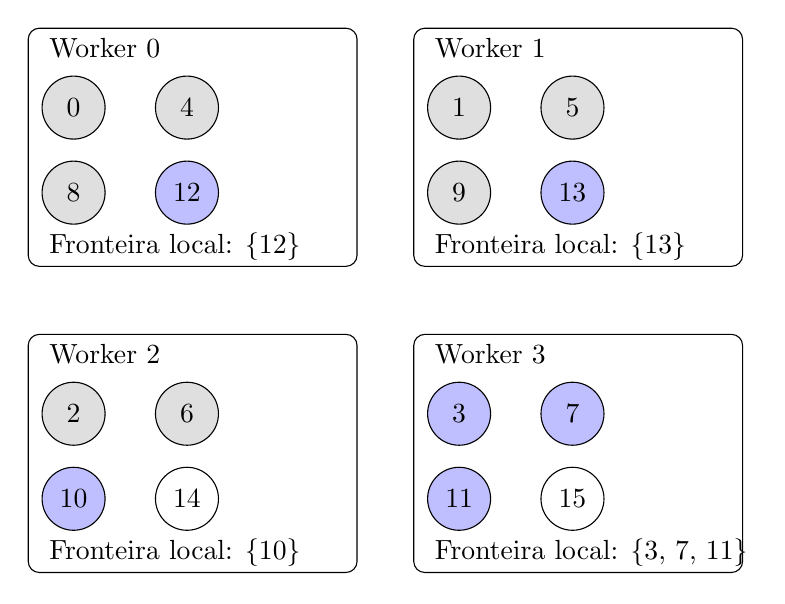
\begin{tikzpicture}[scale=0.72]
  \draw[rounded corners] (-0.8,-0.8) rectangle (5.0,3.4);
  \node[anchor=west] at (-0.6,3.05) {Worker 0};
  \node[visited] at (0,2) {0};
  \node[visited] at (2,2) {4};
  \node[visited] at (0,0.5) {8};
  \node[frontier] at (2,0.5) {12};
  \node[anchor=west] at (-0.6,-0.45) {Fronteira local: \{12\}};

  \draw[rounded corners] (6.0,-0.8) rectangle (11.8,3.4);
  \node[anchor=west] at (6.2,3.05) {Worker 1};
  \node[visited] at (6.8,2) {1};
  \node[visited] at (8.8,2) {5};
  \node[visited] at (6.8,0.5) {9};
  \node[frontier] at (8.8,0.5) {13};
  \node[anchor=west] at (6.2,-0.45) {Fronteira local: \{13\}};

  \draw[rounded corners] (-0.8,-6.2) rectangle (5.0,-2.0);
  \node[anchor=west] at (-0.6,-2.35) {Worker 2};
  \node[visited] at (0,-3.4) {2};
  \node[visited] at (2,-3.4) {6};
  \node[frontier] at (0,-4.9) {10};
  \node[undiscovered] at (2,-4.9) {14};
  \node[anchor=west] at (-0.6,-5.85) {Fronteira local: \{10\}};

  \draw[rounded corners] (6.0,-6.2) rectangle (11.8,-2.0);
  \node[anchor=west] at (6.2,-2.35) {Worker 3};
  \node[frontier] at (6.8,-3.4) {3};
  \node[frontier] at (8.8,-3.4) {7};
  \node[frontier] at (6.8,-4.9) {11};
  \node[undiscovered] at (8.8,-4.9) {15};
  \node[anchor=west] at (6.2,-5.85) {Fronteira local: \{3, 7, 11\}};
\end{tikzpicture}
\caption{Passo 3 da BFS paralela: todos os workers possuem vértices na fronteira.}
\label{fig:bfs-paralela-step3}
\end{figure}

Após o passo 3, apenas os workers 2 e 3 continuam com novos vértices a expandir.

\begin{figure}[H]
\centering
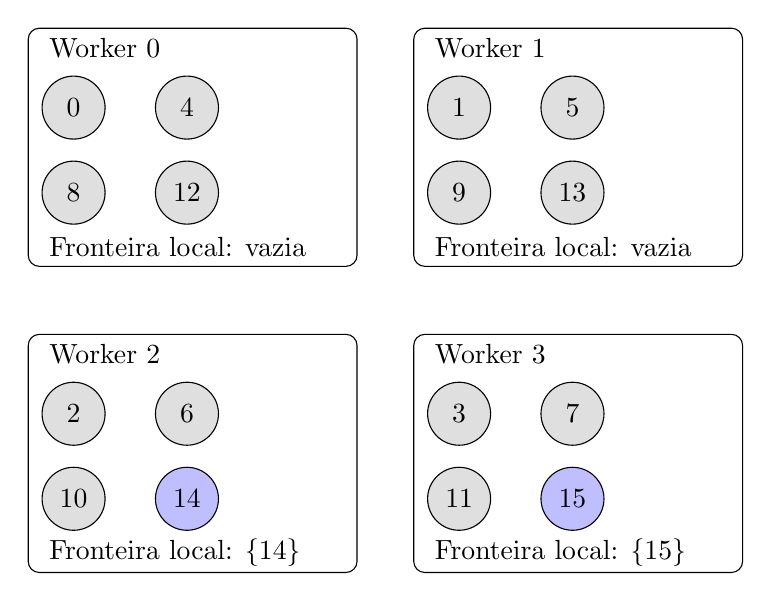
\begin{tikzpicture}[scale=0.72]
  \draw[rounded corners] (-0.8,-0.8) rectangle (5.0,3.4);
  \node[anchor=west] at (-0.6,3.05) {Worker 0};
  \node[visited] at (0,2) {0};
  \node[visited] at (2,2) {4};
  \node[visited] at (0,0.5) {8};
  \node[visited] at (2,0.5) {12};
  \node[anchor=west] at (-0.6,-0.45) {Fronteira local: vazia};

  \draw[rounded corners] (6.0,-0.8) rectangle (11.8,3.4);
  \node[anchor=west] at (6.2,3.05) {Worker 1};
  \node[visited] at (6.8,2) {1};
  \node[visited] at (8.8,2) {5};
  \node[visited] at (6.8,0.5) {9};
  \node[visited] at (8.8,0.5) {13};
  \node[anchor=west] at (6.2,-0.45) {Fronteira local: vazia};

  \draw[rounded corners] (-0.8,-6.2) rectangle (5.0,-2.0);
  \node[anchor=west] at (-0.6,-2.35) {Worker 2};
  \node[visited] at (0,-3.4) {2};
  \node[visited] at (2,-3.4) {6};
  \node[visited] at (0,-4.9) {10};
  \node[frontier] at (2,-4.9) {14};
  \node[anchor=west] at (-0.6,-5.85) {Fronteira local: \{14\}};

  \draw[rounded corners] (6.0,-6.2) rectangle (11.8,-2.0);
  \node[anchor=west] at (6.2,-2.35) {Worker 3};
  \node[visited] at (6.8,-3.4) {3};
  \node[visited] at (8.8,-3.4) {7};
  \node[visited] at (6.8,-4.9) {11};
  \node[frontier] at (8.8,-4.9) {15};
  \node[anchor=west] at (6.2,-5.85) {Fronteira local: \{15\}};
\end{tikzpicture}
\caption{Passo 4 da BFS paralela: apenas os workers 2 e 3 continuam com fronteiras locais.}
\label{fig:bfs-paralela-step4}
\end{figure}

Por fim, a expansão de 14 e 15 não produz novas descobertas. Nesse ponto, a
próxima fronteira fica vazia e a BFS termina.

\begin{figure}[H]
\centering
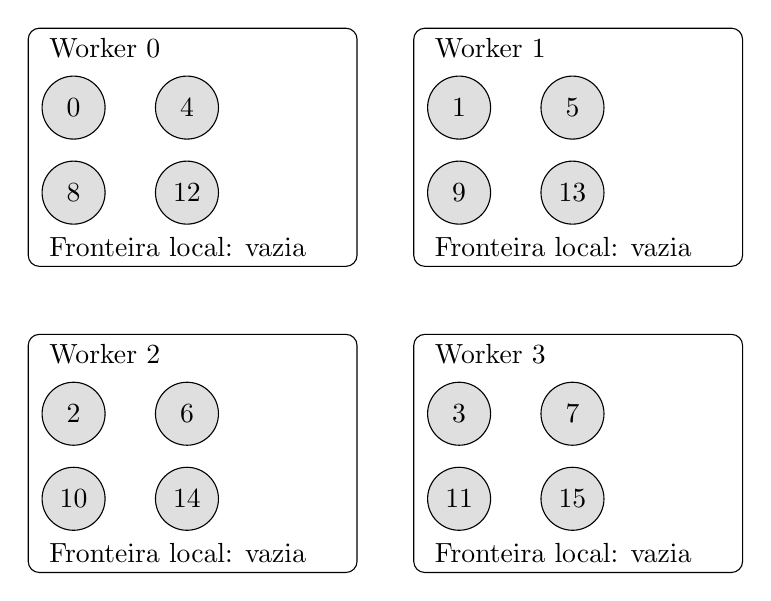
\begin{tikzpicture}[scale=0.72]
  \draw[rounded corners] (-0.8,-0.8) rectangle (5.0,3.4);
  \node[anchor=west] at (-0.6,3.05) {Worker 0};
  \node[visited] at (0,2) {0};
  \node[visited] at (2,2) {4};
  \node[visited] at (0,0.5) {8};
  \node[visited] at (2,0.5) {12};
  \node[anchor=west] at (-0.6,-0.45) {Fronteira local: vazia};

  \draw[rounded corners] (6.0,-0.8) rectangle (11.8,3.4);
  \node[anchor=west] at (6.2,3.05) {Worker 1};
  \node[visited] at (6.8,2) {1};
  \node[visited] at (8.8,2) {5};
  \node[visited] at (6.8,0.5) {9};
  \node[visited] at (8.8,0.5) {13};
  \node[anchor=west] at (6.2,-0.45) {Fronteira local: vazia};

  \draw[rounded corners] (-0.8,-6.2) rectangle (5.0,-2.0);
  \node[anchor=west] at (-0.6,-2.35) {Worker 2};
  \node[visited] at (0,-3.4) {2};
  \node[visited] at (2,-3.4) {6};
  \node[visited] at (0,-4.9) {10};
  \node[visited] at (2,-4.9) {14};
  \node[anchor=west] at (-0.6,-5.85) {Fronteira local: vazia};

  \draw[rounded corners] (6.0,-6.2) rectangle (11.8,-2.0);
  \node[anchor=west] at (6.2,-2.35) {Worker 3};
  \node[visited] at (6.8,-3.4) {3};
  \node[visited] at (8.8,-3.4) {7};
  \node[visited] at (6.8,-4.9) {11};
  \node[visited] at (8.8,-4.9) {15};
  \node[anchor=west] at (6.2,-5.85) {Fronteira local: vazia};
\end{tikzpicture}
\caption{Passo 5 da BFS paralela: a fronteira global fica vazia e a busca termina.}
\label{fig:bfs-paralela-step5}
\end{figure}

Essa sequência visual mostra que a fronteira global da BFS é a união das
fronteiras locais de cada worker. Em uma implementação paralela, cada worker
expande apenas os vértices da sua fronteira local. Quando uma aresta aponta para
um vértice remoto, a atualização precisa ser enviada ao worker dono daquele
vértice, que poderá processá-lo no próximo passo. Essa organização preserva a
ideia de avanço por níveis da BFS, mas distribui o trabalho e a comunicação entre
as unidades de execução disponíveis.

\subsection{BFS em GPU}
GPUs modernas sao otimizadas para executar operacoes computacionalmente intensivas 
com muitos grupos de threads em paralelo e dependem de concorrencia para esconder 
atrasos de memoria. No modelo da NVIDIA, threads sao agrupadas em \textit{warps}, 
que executam uma mesma instrucao sobre dados diferentes, e em blocos de threads, 
que podem compartilhar memoria local no multiprocessador. Esse modelo favorece 
cargas de trabalho com grande quantidade de operacoes independentes e com acesso 
a memoria bem organizado \cite{merrillgpu}.

A BFS e atraente para GPUs porque a expansao de uma fronteira pode expor muito
paralelismo. Em uma mesma iteracao, varios vertices da fronteira atual podem ser
expandidos simultaneamente, e as arestas incidentes a esses vertices tambem podem
ser examinadas em paralelo. Quando a fronteira e grande, ha trabalho suficiente
para ocupar muitos multiprocessadores. Alem disso, a BFS executa pouca computacao
aritmetica por aresta; portanto, seu desempenho depende principalmente de largura
de banda, latencia de memoria, controle de concorrencia e eficiencia na
organizacao das fronteiras \cite{merrillgpu}.

Apesar disso, grafos esparsos tornam a BFS dificil em GPU. O padrao de acesso a
memoria depende da estrutura do grafo, nao de um arranjo regular como em vetores
ou matrizes densas. Ao expandir um vertice, as threads seguem listas de
adjacencia que podem apontar para regioes distantes da memoria. Alem disso, grafos
reais frequentemente possuem distribuicao de grau irregular, alguns vertices tem
poucos vizinhos, enquanto outros concentram muitos. Se uma thread ou um warp recebe 
um vertice de grau muito maior que os demais, ocorre desbalanceamento de carga e 
parte da GPU pode ficar subutilizada \cite{merrillgpu}.

Uma forma simples de paralelizar BFS e fazer cada iteracao inspecionar todos os 
vertices ou todas as arestas do grafo, procurando quais deles pertencem ao nivel atual. 
Essa estrategia se ajusta facilmente ao modelo de dados paralelos da GPU, mas pode
executar trabalho quadratico no pior caso, pois o mesmo grafo e varrido repetidas
vezes ao longo dos niveis da busca. Para grafos com diametro nao trivial, esse
custo se torna alto. Uma implementacao eficiente deve examinar apenas os vertices
e arestas que pertencem as fronteiras ativas de cada iteracao, mantendo custo
linear em relacao ao numero de vertices e arestas, isto e, $O(|V| + |E|)$
\cite{merrillgpu}.

No ponto de vista de desempenho, permitir muitas descobertas duplicadas de um mesmo 
vertice pode gerar trabalho redundante, pois o mesmo vertice pode ser inserido mais 
de uma vez na fronteira e sua lista de adjacencia pode ser expandida repetidamente. 
Por isso, implementacoes em GPU costumam usar mecanismos de filtragem, marcacao e 
remocao local de duplicatas para reduzir esse efeito \cite{merrillgpu}.

Portanto, a BFS em GPU deve equilibrar tres objetivos. Primeiro, preservar a
estrutura por niveis da BFS, garantindo que a proxima fronteira contenha apenas
vertices descobertos a partir da fronteira atual. Segundo, manter eficiencia de
trabalho, evitando varrer o grafo inteiro a cada iteracao. Terceiro, adaptar a
execucao irregular do grafo ao modelo de hardware da GPU, organizando fronteiras,
trabalho e comunicacao de forma a reduzir desbalanceamento, contencao e acessos
ineficientes a memoria
\cite{merrillgpu}.

\section{NVSHMEM}
NVSHMEM e uma biblioteca de comunicao para GPUs NVIDIA baseada no modelo OpenSHMEM. 
O objetivo eh oferecer um espaco de memoria global entre GPUs, onde cada elemento de 
processamento possue uma memoria local, que pode ser enderecado globalmente atraves de
operacoes de comunicacao. O principal diferencial do NVSHMEM e o motivo de ser utilizado
nesse trabalho eh que as operacoes podem ser emitidas diretamente de um kernel CUDA,
sem envolver a CPU \cite{hsunvshmem}.

As unidades de processamento sao divididasaaa em PEs (Process Unit). A biblioteca define
regioes de memoria simetricas, essas regioes sao alocadas coletivamente por todas as PEs.
A simetria permite que uma PE, calcule o endereco logico global correspondente a um
endereco logico local, e um indentificador de PE. O NVSHMEM fornece operacoes remotas
como leituras e escritas, e atomicos.

Pelas suas caracteristicas a biblioteca NVSHMEM e relevante para algoritmos irregulares.
Em aplicacoes densas ou estruturadas, a comunicacao pode ser prevista e agrupada
em mensagens grandes. Em grafos, por outro lado, os destinos das atualizacoes
sao descobertos durante a execucao. Ao expandir uma fronteira de BFS, uma thread
pode visitar uma aresta, identificar que o vertice vizinho pertence a outro PE e
precisar atualizar o estado desse vertice remoto. Com NVSHMEM, essa atualizacao
pode ser expressa diretamente no kernel, usando uma operacao remota ou atomica,
sem retornar primeiro ao host para empacotar mensagens \cite{hsunvshmem}.

\section{MPI}
MPI (\textit{Message Passing Interface}) e um padrao de comunicacao para
programas paralelos em memoria distribuida. Em um programa MPI, a execucao e
organizada em processos independentes, chamados normalmente de ranks. Cada rank
possui seu proprio espaco de enderecamento e troca dados com os demais por meio
de chamadas explicitas de comunicacao. Esse modelo e adequado para clusters,
onde a memoria de uma maquina ou processo nao pode ser acessada diretamente por
outro processo sem uma operacao de comunicacao definida \cite{mpistandard}.

O modelo de MPI se baseia em troca de mensagens. Em comunicacoes ponto a ponto,
um rank envia dados e outro rank recebe esses dados. Operacoes como
\texttt{MPI\_Send} e \texttt{MPI\_Recv} representam esse padrao basico. Tambem
existem versoes nao bloqueantes, como \texttt{MPI\_Isend} e
\texttt{MPI\_Irecv}, que permitem iniciar uma transferencia e continuar a
execucao enquanto a comunicacao progride. Esse tipo de comunicacao e importante
em aplicacoes paralelas porque pode permitir sobreposicao entre computacao e
transferencia de dados.

MPI tambem define operacoes coletivas, nas quais todos os ranks de um
comunicador participam. Exemplos comuns incluem \texttt{MPI\_Barrier}, usada
para sincronizacao, \texttt{MPI\_Bcast}, usada para difundir dados de um rank
para os demais, e \texttt{MPI\_Reduce} ou \texttt{MPI\_Allreduce}, usadas para
combinar valores produzidos localmente por cada rank. Em algoritmos iterativos,
essas operacoes aparecem frequentemente para calcular condicoes globais de
parada, agregar estatisticas ou garantir que todos os processos avancem para a
proxima fase de execucao.

\section{Graph500}
O Graph500 e um benchmark criado para avaliar sistemas de alto desempenho em
cargas de trabalho centradas em grafos e acesso irregular a memoria. O Graph500 
enfatiza movimentacao de dados, comunicacao, acesso indireto a memoria e 
paralelismo irregular \cite{murphygraph500}. Essas caracteristicas 
fazem com que ele seja adequado para estudar algoritmos como BFS em ambientes 
distribuidos e em GPU.

O benchmark define uma entrada sintetica baseada em um grafo gerado por um
modelo do tipo Kronecker/R-MAT. O tamanho do grafo e controlado pelo parametro
\texttt{SCALE}, que define o numero de vertices como $2^{\texttt{SCALE}}$, e
pelo \texttt{edgefactor}, que define a quantidade media de arestas geradas por
vertice. Assim, o numero de arestas cresce proporcionalmente ao numero de
vertices, mas a estrutura gerada nao e regular: ela tende a produzir vertices
com graus muito diferentes, criando hubs e regioes de alta concentracao de
arestas. Esse comportamento e importante porque se aproxima de propriedades
observadas em varios grafos reais \cite{graph500spec}.

O fluxo do Graph500 e organizado em etapas. Primeiro, o benchmark gera uma lista
de arestas, tambem chamada de grafo em tuplas. Nessa forma inicial, cada aresta
e representada apenas por seus dois vertices. Essa representacao e adequada para
geracao e distribuicao inicial dos dados, mas nao e a forma mais eficiente para
executar uma travessia, pois a BFS precisa consultar rapidamente os vizinhos de
cada vertice ativo.

A primeira etapa medida pelo benchmark e conhecida como Kernel 1. Ela consiste
em construir uma estrutura de dados de grafo a partir da lista de arestas. Em
implementacoes de BFS, essa estrutura frequentemente e uma variacao de CSR
(\textit{Compressed Sparse Row}), na qual cada vertice possui um intervalo de
posicoes que aponta para seus vizinhos. Em uma execucao distribuida, essa
construcao tambem precisa decidir qual processo ou PE e responsavel por cada
vertice e por suas listas de adjacencia. Portanto, o Kernel 1 mede a capacidade
do sistema de reorganizar uma entrada irregular em uma estrutura adequada para
travessia \cite{graph500spec}.

Depois da construcao do grafo, o benchmark seleciona um conjunto de raizes para
as execucoes de BFS. A especificacao evita escolher vertices isolados, pois uma
BFS iniciada em um vertice sem arestas nao exercitaria o sistema de forma
representativa. Em geral, sao escolhidas varias raizes, e a BFS e executada uma
vez para cada uma delas. Isso reduz a chance de o resultado depender apenas de
uma origem especifica e permite calcular estatisticas como minimo, maximo, media
e mediana de desempenho.

A segunda etapa principal e o Kernel 2, chamado de \textit{Search}. Nessa etapa,
o benchmark executa BFS a partir de cada raiz selecionada. O resultado esperado
nao e apenas a ordem de visita dos vertices, mas uma arvore de predecessores.
Cada vertice alcancavel deve registrar um pai valido, isto e, um vertice que o
descobriu no nivel anterior da busca. Vertices nao alcancaveis a partir da raiz
devem permanecer sem predecessor. Essa representacao por predecessores e usada
posteriormente para validar a corretude da BFS \cite{graph500spec}.

A validacao e uma parte essencial do Graph500. Uma implementacao nao pode apenas
produzir um tempo de execucao baixo; ela precisa demonstrar que a arvore de BFS
gerada e correta. A validacao verifica propriedades como: a raiz aponta para si
mesma, vertices visitados possuem predecessores validos, as arestas da arvore
existem no grafo, e os niveis respeitam a propriedade da BFS. Essa etapa e
especialmente importante em implementacoes paralelas, nas quais varias threads
ou processos podem tentar descobrir o mesmo vertice ao mesmo tempo.

A principal metrica de desempenho reportada pelo Graph500 e TEPS
(\textit{Traversed Edges Per Second}). Essa metrica representa quantas arestas
sao atravessadas por segundo durante a BFS. Como a BFS executa pouca computacao
aritmetica por aresta, TEPS e uma metrica mais apropriada do que operacoes de
ponto flutuante por segundo. Ela reflete melhor a capacidade do sistema de
percorrer estruturas irregulares, acessar memoria, comunicar descobertas remotas
e sincronizar a execucao distribuida.

\bibliographystyle{plain}
\bibliography{bibliografia}
\end{document}
